\section{Durchführung}
\label{sec:Durchfuehrung}
Für den Versuch wird als Anodenmaterial Kupfer verwendet und über eine Blende der Röntgenstrahl auf das Material gelenkt.
Die Elektronen werden mit einer Beschlenigungsspannung von  $35 \text{keV}$ beschleunigt.
Es lassen sich sowohl der verwendete LiF Kristall als auch das Geiger Müller Zählrohr im Bezug auf den Strahl drehen.
Für den letzten Teil des Versuchs lässt sich zwischen dem Kristall und dem Zählrohr eine Probe anbringen um die Absorption zu messen.
\begin{figure}
    \centering
    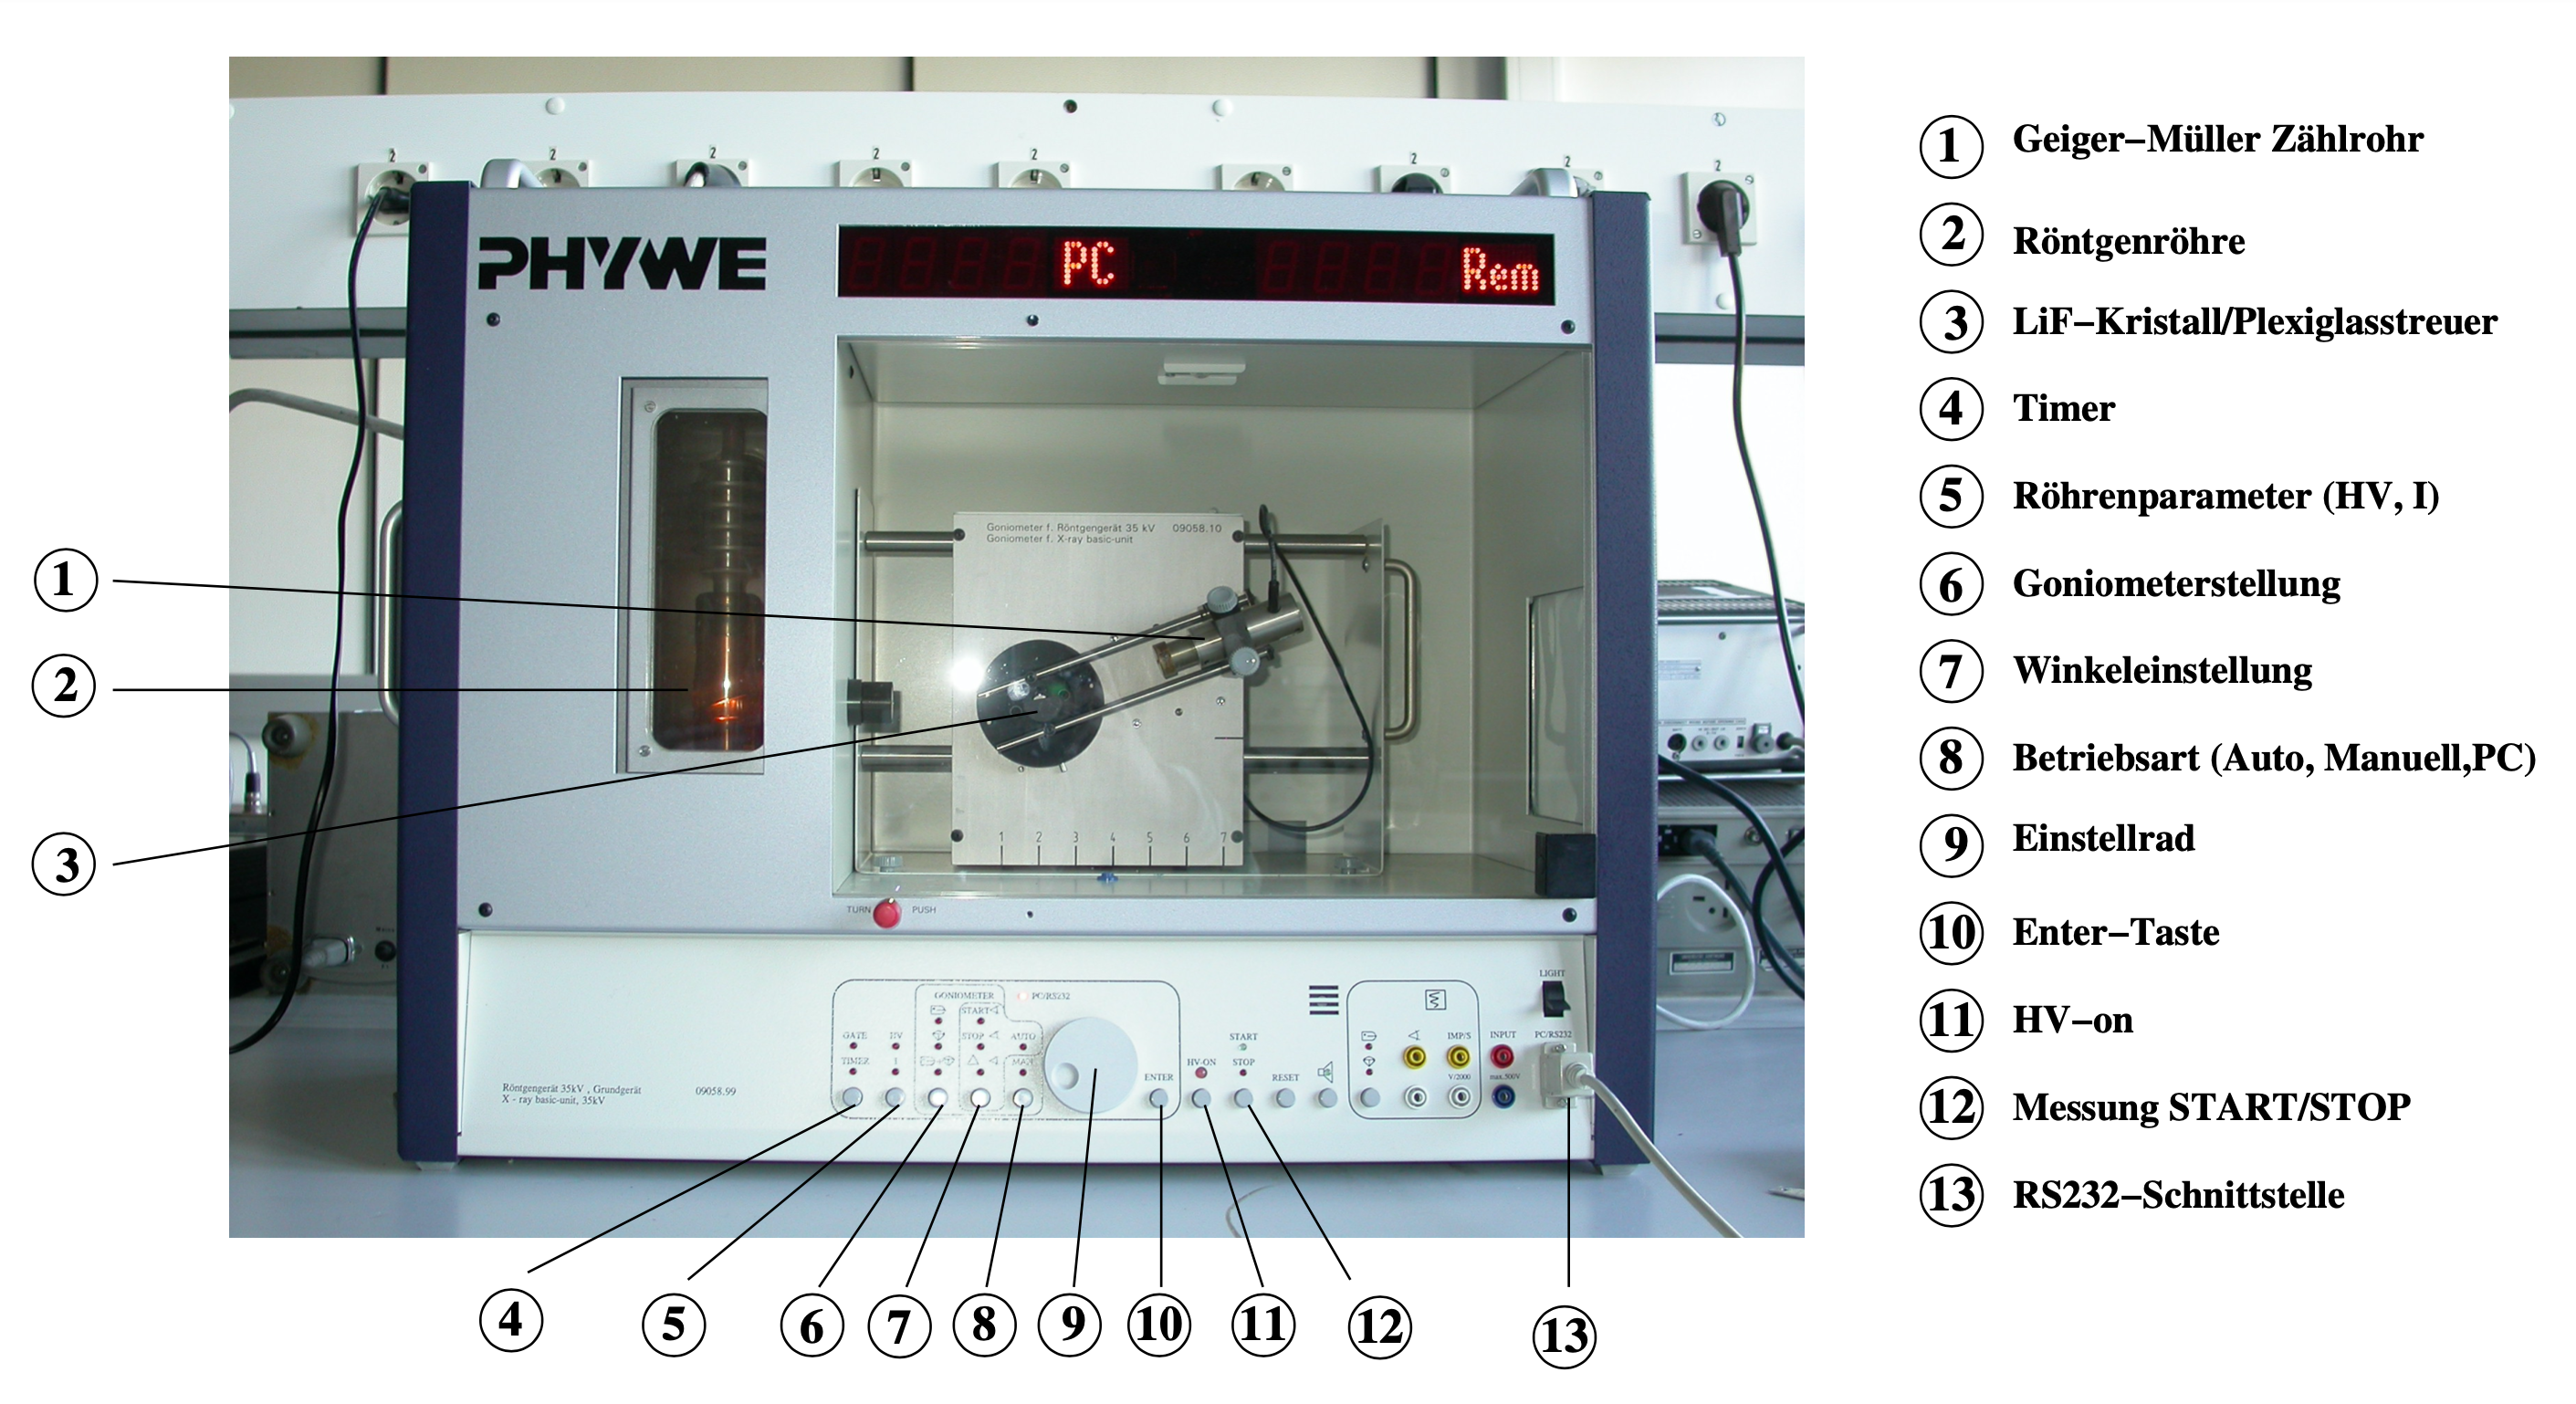
\includegraphics[width=0.7\textwidth]{bilder/Versuchsaufbau.png}
    \caption{Ein Foto des Versuchsaufbaus mit Beschriftung der Komponenten. (Quelle \cite{Anleitung})}
    \label{fig:Versuchsaufbau}
\end{figure}

\subsection{Braggbedingung überprüfen}
Für die Überprüfung der Braggbedingung wird der LiF Kristall in einen festen Winkel $\alpha = 14°$ zum Photonenstrahl gebracht.
Nun wird das Geiger Müller Zählrohr Über das Winkelintervall von 26° bis 30° in $\Delta \alpha = 0,1°$ Schritten mit einer Integrationszeit von $\Delta t = 5 \text{s}$ gedreht.
Aus den Werten lässt sich das Intensitätsmaximum auslesen und mit der Braggbedingung vergleichen.
\subsection{Kupfer Emissionsspektrum}
Um das Emissionsspektrum von Kupfer zu untersuchen wird nun von $8°$ bis $25°$ der Kristall gedreht und jeweils über eine Integrationszeit von $10 \text{s}$ in $\Delta \theta = 0,1°$ Schritten die Intensität aufgenommen.
\subsection{Absorptionsspektren}
Um die K-Kantne verschiedener Materialien und damit die Rydbergenergie zu bestimmen werden die Absorptionsspektren der Materialien aufgenommen.
Dazu wird zwischen dem LiF Kristall und dem Zählrohr eine Metallprobe eingesetzt und über eine Integrationszeit von zwanzig Sekunden und $\Delta \theta = 0,1°$ das entsprechende Spektrum aufgenommen.
Die Spektren wurden für die Materialien Brom, Gallium, Rubidium,Strontium, Zink und Zirkonium aufgenommen.
Aus dem Spektrum lässt sich an den speziellen Stellen die K-Kante erkennen und ablesen.